\chapter{The Simple Symmetric Random Walk}

\section{The Model}

Let $X_1,X_2,X_3,\ldots$ be i.i.d.\ random variables such that
\begin{equation}
X_i = \begin{cases}
1 & \mbox{with probability } \frac{1}{2} \;,\\
-1 & \mbox{with probability } \frac{1}{2} \;.
\end{cases}
\end{equation}
The sequence of random variables $\left(S_n\right)_{n=0}^\infty$ defined as $S_0\equiv 0$ and for $n\geq 1$
\begin{equation}
S_n \coloneqq X_1+\cdots+X_n \;,
\end{equation}
is called the one-dimensional Simple Symmetric Random Walk (SSRW).

\section{Descriptive Statistics}

\textbf{Question:} What is the maximum value of $S_n$?\\
\textbf{Answer:} $n$.\\

\medskip

\noindent\textbf{Question:} What is the minimum value of $S_n$?\\
\textbf{Answer} $-n$.\\

\medskip 

\noindent\textbf{Question:} What is the average value (i.e., the expectation) of $S_n$?\\
\textbf{Answer:} Average value of $S_n$ is $0$ as the following calculation shows:
\begin{equation}
\Exp*{S_n}=\Exp*{X_1+\cdots+X_n}=\Exp*{X_1}+\cdots+\Exp*{X_n}=0+\cdots+0=0\;.
\end{equation}
Here we do not need the assumption that $X_i$s are independent. We use that $\Exp*{X_i}=0$ for each $i$:
\begin{equation}
\Exp*{X_i}=1\cdot\frac{1}{2}+(-1)\cdot\frac{1}{2}=0\;.
\end{equation}

\medskip

\noindent\textbf{Question:} What is the variance of $S_n$?\\
\textbf{Answer:}
\begin{equation}
\var*{S_n}=\var*{X_1}+\cdots+\var*{X_n}=1+\cdots+1=n\;.
\end{equation}
Here we use the assumption that $X_i$s are independent; otherwise there would be the covariance terms. 

\begin{tcolorbox}[title={Skip on first reading}]
Technically speaking, we are only using that pairwise covariances are $0$, which follows from the assumption of independence, but is a much weaker condition. 
\tcblower
\begin{itemize}
    \item Example of two random variables which are not independent but their covariance is $0$: $X$ and $X^2$ where $X\sim\mathcal{N}(0,1)$.
    \item Example of three random variables which pairwise independent but not independent jointly: $XY,YZ,ZX$ where
    $X,Y,Z$ are i.i.d.\ with $\Prob*{X=1}=\Prob*{X=-1}=1/2$. 
\end{itemize}
\end{tcolorbox}

Above we used $\var*{X_i}=1$ as the following calculation shows:
\begin{equation}
\var*{X_i}=\Exp*{X_i^2}-\Bigl(\Exp*{X_i}\Bigr)^2=\Exp*{1}-0^2=1\;.
\end{equation}

\begin{tcolorbox}[title={Skip on first reading}]
Consider two random variables 
$X$ and $Y$. Assume $\Exp*{X^2}<\infty$
and $\Exp*{Y^2}<\infty$.
\tcblower
If $X$ and $Y$ are independent then 
$\cov*{X,Y}=0$. But the converse is
not true. The converse is true in a
very important situation: when $(X,Y)$
is multivariate-normal. In this situation,
$\cov{X,Y}=0$ implies $X$ and $Y$ are independent. 
\end{tcolorbox}

\section{Exact Distribution}

\textbf{Question:} $X_i$s are similar to Bernoulli random variables. $S_n$ should be similar to a Binomial random variable. Can we make it precise?\\
\noindent\textbf{Answer}: 
\begin{equation}
\frac{n+S_n}{2}\sim\mathrm{Binomial}(n,\frac{1}{2})\;.
\end{equation}
We observe that
\begin{equation}
\frac{1+X_i}{2}=
\begin{cases}
1 & \mbox{with probability } \frac{1}{2} \;,\\
0 & \mbox{with probabiluty } \frac{1}{2} \;.
\end{cases}
\end{equation}
Therefore $(1+X_i)/2$ is a $\mathrm{Bernoulli}(1/2)$
random variable. Therefore
\begin{equation}
\frac{1+X_1}{2} + 
\frac{1+X_2}{2} +
\cdots +
\frac{1+X_n}{2}
=\frac{n+S_n}{2}
\sim\mathrm{Binomial}(n,1/2)\;.
\end{equation}

\section{Approximate Distribution}

From SLLN we get
\begin{equation}
\frac{S_n}{n}\to 0 
\end{equation}
almost surely. From CLT we get
\begin{equation}
\frac{S_n}{\sqrt{n}}\to N(0,1)
\end{equation}
in distribution i.e., for all $x\in\real$
\begin{equation}
\Prob*{S_n\leq x\sqrt{n}}\to\int_{-\infty}^x
\frac{1}{\sqrt{2\pi}}e^{-t^2/2}dt.
\end{equation}

\section{Path Counting}

A path from $(0,0)$ to $(n,x)$ is a sequence $s_0,s_1,\ldots,s_n$ such that $s_0=0$, $s_n=x$, and for each $i$, $|s_{i+1}-s_{i}|=1$. Note that $n$ and $x$ must have same parity for there to be any path from $(0,0)$ to $(n,x)$.

\noindent \textbf{Question:} How many paths are there from $(0,0)$ to $(n,x)$?\\
\noindent\textbf{Answer:} Let us denote the number of paths from $(0,0)$ to $N_{n,x}$ by $N_{n,x}$. Thus $N_{n,x}=0$ if $n$ 
and $x$ are of opposite parity. Now suppose $n$ and $x$ have the same parity. Suppose a path from $(0,0)$ to $(n,x)$ consists of $p$ moves which are $+1$s ($i+1$'th move is $+1$ if $s_{i+1}-s_i=1$ ) and $q$ moves which are $-1$s ($i+1$'th move is $-1$ if $s_{i+1}-s_i=-1$). Then 
\begin{equation}
n = p+q.
\end{equation}
and
\begin{equation}
x = p-q.
\end{equation}
Solving for $p$ and $q$ yields $p=(n+x)/2$ and $q=(n-x)/2$. Clearly there is a bijection between paths from $(0,0)$ to $(n,x)$ and arrangements of $p$ $+1$s and $q$ $-1$s. Therefore
\begin{equation}
N_{n,x} 
= \binom{p+q}{p} 
= \binom{p+q}{q} 
= \binom{n}{\frac{n+x}{2}}
= \binom{n}{\frac{n-x}{2}}\;.
\end{equation}

\begin{proposition}[Formula for the Number of Simple Random Walk Paths]
Let $N_{n,x}$ denote the number of paths from $(0,0)$ to $(n,x)$. Then for $n$ and $x$ having the same parity and $x\in[-n,n]$ we have
\begin{equation}
N_{n,x} 
= \binom{n}{\frac{n+x}{2}}
= \binom{n}{\frac{n-x}{2}}\;.
\end{equation}
\end{proposition}

\newpage

\fancyhead[L]{\fcolorbox{red}{yellow}{Lecture 2. February 24, 2025}}

\section{The Reflection Principle}

\begin{theorem}[The Reflection Principle]
$b>a\geq 0$. $\alpha>0$. $\beta>0$. $A=(a,\alpha)$. $B=(b,\beta)$. $A^\prime=(a,-\alpha)$. The number of paths from $A$ to $B$ which touch or cross the $x$-axis equals number of all paths from $A^\prime$ to $B$.
\end{theorem}

\begin{center}
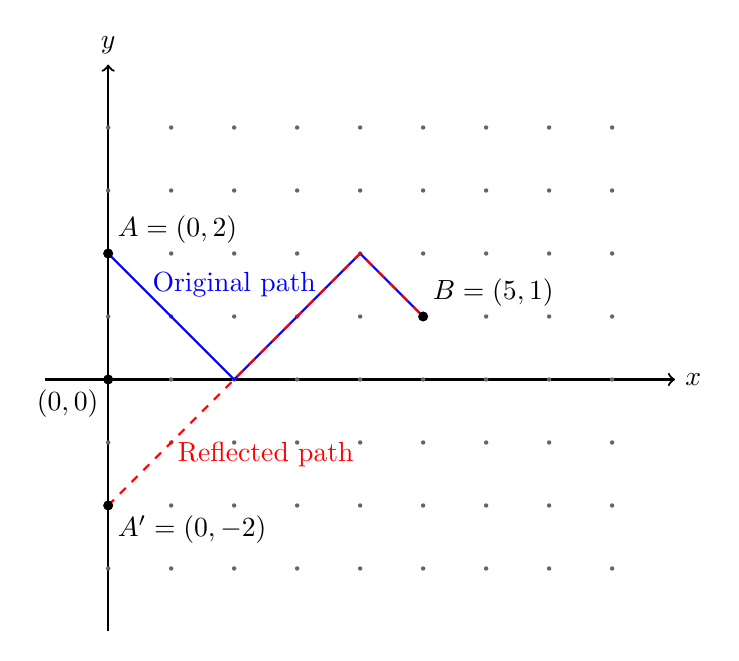
\begin{tikzpicture}[scale=0.8]
  % Axes
  \draw[thick,->] (-1,0) -- (9,0) node[right] {$x$};
  \draw[thick,->] (0,-4) -- (0,5) node[above] {$y$};

  % Grid points for better understanding
  \foreach \x in {0,...,8}
    \foreach \y in {-3,...,4}
      \fill[black!60] (\x,\y) circle (1pt);

  % Original path: up-up-down-up-down
  \draw[thick, blue] (0,2) -- (1,1) -- (2,0) -- (3,1) -- (4,2) -- (5,1);

  % Reflected path: up-up-down-down-up (touches x-axis)
  \draw[thick, red, dashed] (0,-2) -- (1,-1) -- (2,0) -- (3,1) -- (4,2) -- (5,1);
  
  % Reflected portion shown flipped below x-axis
  %\draw[thick, red, dashed] (3,1) -- (4,0) -- (5,1);
  %\draw[thick, red] (3,-1) -- (4,0) -- (5,1);

  % Dotted line showing reflection
  %\draw[dashed, gray] (3,1) -- (3,-1);

  % Labels
  \node[blue] at (2.0,1.5) {Original path};
  \node[red] at (2.5,-1.2) {Reflected path};

  % Mark start and end points
  \filldraw[black] (0,0) circle (2pt) node[below left] {$(0,0)$};
  \filldraw[black] (5,1) circle (2pt) node[above right] {$B=(5,1)$};
  \filldraw[black] (0,2) circle (2pt) node[above right] {$A=(0,2)$};
  \filldraw[black] (0,-2) circle (2pt) node[below right] {$A^\prime=(0,-2)$};
  
\end{tikzpicture}
\end{center}

\section{The Ballot Problem}

\begin{theorem}[The Ballot Problem]
Let $n$ and $x$ be positive integers. There are exactly $\frac{x}{n}N_{n,x}$ paths $(s_1,\ldots,s_n=x)$ from the origin to the point $(n,x)$ such that $s_1>0,\ldots,s_n>0$.
\end{theorem}

\begin{figure}[h]
\centering
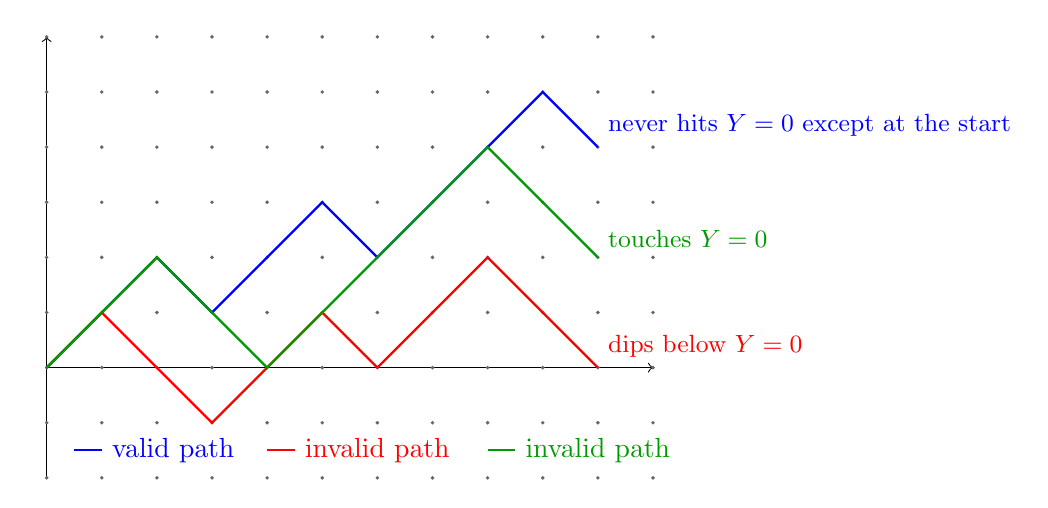
\begin{tikzpicture}[scale=0.7]
    \draw[->] (0,0) -- (11,0) node[below] {};
    \draw[->] (0,-2) -- (0,6) node[left] {};
    % Grid points
    \foreach \x in {0,...,11}
        \foreach \y in {-2,...,6}
            \fill[black!60] (\x,\y) circle (1pt);
    % Example good path
    \coordinate (P0) at (0,0);
    \coordinate (P1) at (1,1);
    \coordinate (P2) at (2,2);
    \coordinate (P3) at (3,1);
    \coordinate (P4) at (4,2);
    \coordinate (P5) at (5,3);
    \coordinate (P6) at (6,2);
    \coordinate (P7) at (7,3);
    \coordinate (P8) at (8,4);
    \coordinate (P9) at (9,5);
    \coordinate (P10) at (10,4);

    \draw[thick,blue] (P0) -- (P1) -- (P2) -- (P3) -- (P4) -- (P5) -- (P6) -- (P7) -- (P8) -- (P9) -- (P10) node[above right] {\small never hits $Y=0$ except at the start};

    % Example bad path (crosses below 0)
    \coordinate (Q0) at (0,0);
    \coordinate (Q1) at (1,1);
    \coordinate (Q2) at (2,0);
    \coordinate (Q3) at (3,-1);
    \coordinate (Q4) at (4,0);
    \coordinate (Q5) at (5,1);
    \coordinate (Q6) at (6,0);
    \coordinate (Q7) at (7,1);
    \coordinate (Q8) at (8,2);
    \coordinate (Q9) at (9,1);
    \coordinate (Q10) at (10,0);

    \draw[thick,red] (Q0) -- (Q1) -- (Q2) -- (Q3) -- (Q4) -- (Q5) -- (Q6) -- (Q7) -- (Q8) -- (Q9) -- (Q10) node[above right] {\small dips below $Y=0$};

    % Example bad path (touches 0)
    \coordinate (R0) at (0,0);
    \coordinate (R1) at (1,1);
    \coordinate (R2) at (2,2);
    \coordinate (R3) at (3,1);
    \coordinate (R4) at (4,0);
    \coordinate (R5) at (5,1);
    \coordinate (R6) at (6,2);
    \coordinate (R7) at (7,3);
    \coordinate (R8) at (8,4);
    \coordinate (R9) at (9,3);
    \coordinate (R10) at (10,2);

    \draw[thick,green!60!black] (R0) -- (R1) -- (R2) -- (R3) -- (R4) -- (R5) -- (R6) -- (R7) -- (R8) -- (R9) -- (R10) node[above right] {\small touches $Y=0$};

    \draw[thick,blue] (0.5,-1.5) -- (1,-1.5) node[right] {valid path};
    \draw[thick,red] (4,-1.5) -- (4.5,-1.5) node[right] {invalid path};
    \draw[thick,green!60!black] (8,-1.5) -- (8.5,-1.5) node[right] {invalid path};
\end{tikzpicture}
\end{figure}

\begin{proof}
From all paths from $(1,1)$ to $(n,x)$ 
subtract paths from $(1,1)$ to $(n,x)$
that touch or cross $Y=0$. Number of paths
from $(1,1)$ to $(n,x)$ that touch or cross $Y=0$ is equal to number of paths from $(1,-1)$ to $(n,x)$.
\begin{align*}
& N_{n-1,x-1}-N_{n-1,x+1} \\[1em]
={} & \binom{n-1}{\frac{n+x}{2}-1}
- \binom{n-1}{\frac{n+x}{2}} \\[1em]
={} & \frac{(n-1)!}{(\frac{n+x}{2}-1)!(n-\frac{n+x}{2})!}
- \frac{(n-1)!}{(\frac{n+x}{2})!(n-\frac{n+x}{2})!}\\[1em]
={} & \frac{(n-1)!}{(\frac{n+x}{2}-1)!(n-\frac{n+x}{2}-1)!}
\Bigl(\frac{1}{\frac{n+x}{2}}
-\frac{1}{n-\frac{n+x}{2}}\Bigr)\\[1em]
={} & \frac{(n-1)!}{(\frac{n+x}{2}-1)!(n-\frac{n+x}{2}-1)!}
\frac{x}{\frac{n+x}{2}\bigl(n-\frac{n+x}{2}\bigr)}\\[1em]
={} & \frac{(n-1)!}{(\frac{n+x}{2})!(n-\frac{n+x}{2})!}
x\\[1em]
={} & \frac{n!}{(\frac{n+x}{2})!(n-\frac{n+x}{2})!}
\frac{x}{n}\\[1em]
={} & N_{n,x}\frac{x}{n}\;.\\[1em]
\end{align*}
\end{proof}

\section{Catalan Numbers}

How many paths are there from $(0,0)$ to $(2n,0)$ that do not go below the $X$-axis? 

\begin{figure}[h]
\centering
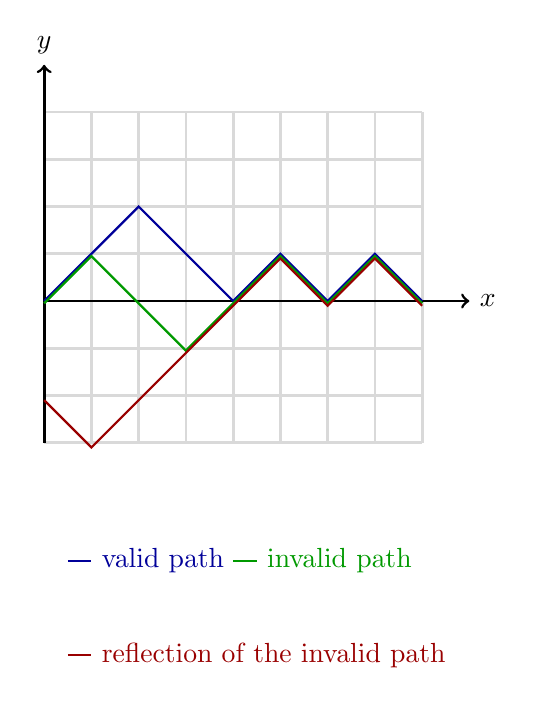
\begin{tikzpicture}[scale=0.6, line width=1pt]
% Draw grid (optional)
  \foreach \x in {0,...,8}
    \draw[gray!30] (\x,-3) -- (\x,4);
  \foreach \y in {-3,...,4}
    \draw[gray!30] (0,\y) -- (8,\y);

  % Draw axes
  \draw[->] (0,0) -- (9,0) node[right] {\(x\)};
  \draw[->] (0,-3) -- (0,5) node[above] {\(y\)};
  
  % Draw Catalan path steps
  \draw[blue!60!black, thick]
    (0,0) -- (1,1)
    -- (2,2)
    -- (3,1)
    -- (4,0)
    -- (5,1)
    -- (6,0)
    -- (7,1)
    -- (8,0);
\begin{scope}[shift={(0,-0.05)}]
\draw[green!60!black, thick]
    (0,0) -- (1,1)
    -- (2,0)
    -- (3,-1)
    -- (4,0)
    -- (5,1)
    -- (6,0)
    -- (7,1)
    -- (8,0);
\end{scope}
\begin{scope}[shift={(0,-0.1)}]
\draw[red!60!black, thick]
    (0,-2) -- (1,-3)
    -- (2,-2)
    -- (3,-1)
    -- (4,0)
    -- (5,1)
    -- (6,0)
    -- (7,1)
    -- (8,0);
\end{scope}
\draw[thick,blue!60!black] (0.5,-5.5) -- (1,-5.5) node[right] {valid path};
\draw[thick,green!60!black] (4,-5.5) -- (4.5,-5.5) node[right] {invalid path};
\draw[thick,red!60!black] (0.5,-7.5) -- (1,-7.5) node[right] {reflection of the invalid path};
\end{tikzpicture}
\end{figure}
Number of paths from $(0,0)$ to $(2n,0)$ is
\[
\binom{2n}{n}.
\]
From this we need to subtract paths that touch or cross the $X=-1$ line. We can calculate this using reflection principle. By reflection principle this is same as number of paths from $(0,-2)$ to $(2n,0)$, which is
\[
\binom{2n}{n-1}.
\]
The difference is
\begin{align*}
& \binom{2n}{n}-\binom{2n}{n-1} \\
={} & \frac{(2n)!}{n!n!}-\frac{(2n)!}{(n+1)!(n-1)!} \\
={} & \frac{(2n)!}{n!(n-1)!}\left(\frac{1}{n}-\frac{1}{n+1}\right)\\
={} & \frac{(2n)!}{n!(n-1)!}\frac{1}{n(n+1)}\\
={} & \frac{(2n)!}{n!n!}\frac{1}{n+1}\\
={} & \frac{1}{n+1}\binom{2n}{n}\;.
\end{align*}

\section{The Main Lemma}

\begin{theorem}[The "Main Lemma" from \citeauthor{Feller1}]

Number of paths of length $2n$ starting from $(0,0)$ that do not touch the $X$-axis is equal to the number of paths that start from $(0,0)$ and end at $(2n,0)$. Equivalently,
\[
\Prob*{S_1\neq 0, S_2\neq 0,\ldots, S_{2n}\neq 0} = \Prob*{S_{2n}=0}\;.
\]    
\end{theorem}

\begin{proof}
Number of paths from $(0,0)$ to $(2n,0)$ is 
\[
N_{2n,0}=\binom{2n}{n}\;.
\]
We have to show that number of paths $(s_0,s_1,\ldots,s_{2n})$ such that $s_1\neq 0,s_2\neq 0,\ldots,s_{2n}\neq 0$ is also $\binom{2n}{n}$. So let us count the number of such paths. By symmetry the number of paths with $s_1\neq 0,\ldots,s_{2n-1}\neq 0,s_{2n}>0$ is same as number of paths with $s_1\neq 0,\ldots,s_{2n-1}\neq 0,s_{2n}<0$. So it is enough to show that number of paths with $s_1\neq 0,\ldots,s_{2n-1}\neq 0,s_{2n}>0$ is $\frac{1}{2}\binom{2n}{n}$. If $s_{2n}>0$, then $s_{2n}=2r$ for some $r=1,\ldots,n$. We will count number of paths $s_1\neq 0,\ldots,s_{2n-1}\neq 0,s_{2n}=2r$ and then sum over $r=1,\ldots,n$. For a path satisfying $s_1\neq 0,\ldots,s_{2n-1}\neq 0,s_{2n}=2r$ we must have $s_1=1$ and $s_2>0,s_3>0,\ldots,s_{2n-1}>0$. Using the reflection principle as we did in the Ballot problem, number of paths from $(1,1)$ to $(2n,2r)$ that do not touch or cross the time axis is 
\[
N_{2n-1,2r-1}-N_{2n-1,2r+1}.
\]
Now if we sum over $r=1,\ldots,n$ we get a telescoping sum:
\begin{align*}
& \sum_{r=1}^{n} \Bigl( N_{2n-1,2r-1}-N_{2n-1,2r+1} \Bigr) \\[1em]
={} & \Bigl(N_{2n-1,1}-N_{2n-1,3}\Bigr)
+ \Bigl(N_{2n-1,3}-N_{2n-1,5}\Bigr)
+ \cdots + 
\Bigl( N_{2n-1,2n-1} - \underbrace{N_{2n-1,2n+1}}_{=0}\Bigr) \\[1em]
={} & N_{2n-1,1} \\[1em]
={} & \binom{2n-1}{\frac{2n-1+1}{2}} \\[1em]
={} & \binom{2n-1}{n} \\[1em]
={} & \frac{(2n-1)!}{n!(n-1)!} \\[1em]
={} & \frac{1}{2}\frac{(2n)!}{n!n!}\\[1em]
={} & \frac{1}{2}\binom{2n}{n}\;.
\end{align*}
\end{proof}

\newpage

\fancyhead[L]{\fcolorbox{red}{yellow}{Lecture 3. March 3, 2025}}

\section{Last Visit to $0$}

For $n\geq 1$, define
\[
L_n \coloneqq \max\Set*{ k \in\Set*{0,1,2,\ldots,n} \given S_k = 0}\;.
\]
Thus $L_n$ denotes the last time the random walk visits $0$ by time $n$. The minimum possible value of $L_n$ is $0$. The maximum possible value of $L_n$ is $n$ if $n$ is even, and $n-1$ if $n$ is odd. $L_n$ is always even.


\begin{theorem}[The Arc-Sine Law for Last Visits]\label{thm:arcsinelaw}
$L_n/n$ converges in distribution to the arc-sine law:
\[
\Prob*{\frac{L_n}{n}\leq x}\to\frac{2}{\pi}\arcsin(\sqrt{x})\;.
\]
This distribution function has density
\[
f(x)=\frac{1}{\pi}\frac{1}{\sqrt{x(1-x)}}
\]
\end{theorem}

\begin{figure}[h]
\centering
% \includegraphics[width=0.7\linewidth]{Figures/arcsine.png}
\caption{Arc-sine law - illustration.}
\label{fig:arc-sine-law-illustration}
\end{figure}

% \begin{lstlisting}
% N = 2000
% T = 300
% X = matrix(0,nr=N,nc=T)
% S = matrix(0,nr=N,nc=T)
% LastVisit = matrix(0,nr=N,nc=1)
% for(i in 1:N){
%   X[i,1] = 2*rbinom(1,1,0.5)-1
%   S[i,1] = X[i,1]
%   LastVisit[i] = 0
%   for(j in 2:T){
%     X[i,j] = 2*rbinom(1,1,0.5)-1
%     S[i,j] = S[i,j-1] + X[i,j]
%     if(S[i,j]==0){
%       LastVisit[i] = j
%     }
%   }
% }
% ScaledLastVisit = LastVisit[,1]/T

% fun <- function(t){
%   return((1/pi)*(t*(1-t))^(-0.5)) 
% }

% hist(ScaledLastVisit,breaks=40,freq=FALSE,
% main="Histogram of Last Visit",asp=1,ylim=c(0,2))
% curve(fun, add = TRUE, col = 2, lwd = 3)
% \end{lstlisting}

\begin{proposition}[Exact Distribution of $L_n$]    
Let $N=n/2$ if $n$ is even. Let $N=(n-1)/2$ if $n$ is odd. Then
\[
\Prob*{L_n=2m} = \frac{1}{2^{2N}}\binom{2m}{m}\binom{2N-2m}{N-m}\;.
\]    
\end{proposition}

\begin{proof}
Consider the case that $n$ is even, so $n=2N$.
We want the probability that for a path of length $2N$,
the last visit occurs at $2m$. Number of paths from $(0,0)$ to $(2m,0)$ is 
\[
\binom{2m}{m}.
\]
Number of paths from $(2m,0)$ to $(2n,0)$ that do not touch the $X$-axis is
\[
\binom{2n-2m}{n-m}.
\]
Hence we get the result. For the case $n$ is odd, we can say $\Prob*{L_n=2m}=\Prob*{L_{n-1}=2m}$ and we can apply the case of even $n$ as now $n-1$ is even.
\end{proof}

\begin{center}
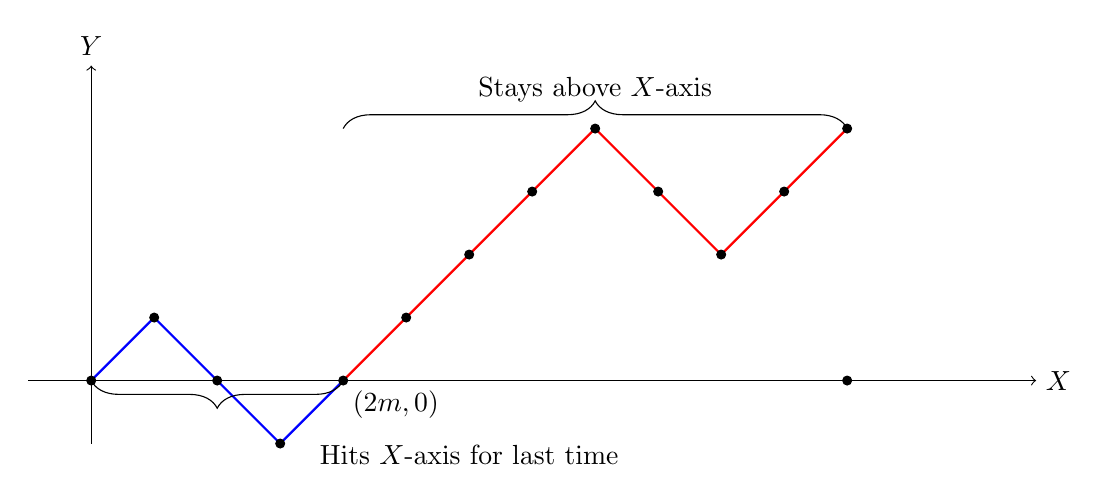
\begin{tikzpicture}[scale=0.8]
  % Axes
  \draw[->] (-1,0) -- (15,0) node[right] {$X$};
  \draw[->] (0,-1) -- (0,5) node[above] {$Y$};

  % Parameters
  % Define the walk: sequence of (up, down) steps
  \coordinate (A0) at (0,0);
  \coordinate (A1) at (1,1);
  \coordinate (A2) at (2,0);
  \coordinate (A3) at (3,-1);
  \coordinate (A4) at (4,0); % last time hitting x-axis (2m = 4)
  \coordinate (B4) at (4,4);
  \coordinate (A5) at (5,1);
  \coordinate (A6) at (6,2);
  \coordinate (A7) at (7,3);
  \coordinate (A8) at (8,4);
  \coordinate (A9) at (9,3);
  \coordinate (A10) at (10,2);
  \coordinate (A11) at (11,3);
  \coordinate (A12) at (12,4);
  \coordinate (B12) at (12,0); 

  % Original path
  \draw[thick, blue] (A0) -- (A1) -- (A2) -- (A3) -- (A4);

  % Path after last return to x-axis
  \draw[thick, red] (A4) -- (A5) -- (A6) -- (A7) -- (A8) -- (A9) -- (A10) -- (A11) -- (A12);

  % Points
  \foreach \pt in {A0,A1,A2,A3,A4,A5,A6,A7,A8,A9,A10,A11,A12,B12}
    \filldraw (\pt) circle (2pt);

  % Label the key point
  \node[below right] at (A4) {$(2m, 0)$};

  % Braces to indicate walk segments
  \draw[decorate,decoration={brace,mirror,amplitude=10pt}]
    (A0) -- (A4) node[pos=1.5,below=20pt] {Hits $X$-axis for last time};

  \draw[decorate,decoration={brace,amplitude=10pt}]
    (B4) -- (A12) node[midway,above=6pt] {Stays above $X$-axis};

\end{tikzpicture}
\end{center}

This result yields a nice, not-so-obvious combinatorial identity, which we record in the appendix.

\begin{proposition}[Approximate Distribution of $L_n$]    
\[
\Prob*{L_n=2m} \approx \frac{1}{\pi}\frac{1}{\sqrt{m(N-m)}}\;.
\]    
\end{proposition}

\begin{proof}
This follows by applying Stirling's approximation
\[
n! \approx \sqrt{2\pi n} \left( \frac{n}{e} \right)^n
\]
\end{proof}

Now we can give a proof of Theorem~\ref{thm:arcsinelaw}. Skip this for first reading. Come back to this after reading convergence in distribution.

\begin{proof}[Proof of Theorem~\ref{thm:arcsinelaw}]    
Consider $0<a<b<1$.
\begingroup
%\addtolength{\jot}{1em}
\begin{align*}
& \Prob*{\frac{L_n}{n}\in(a,b]} \\
={} & \Prob*{na<L_n\leq nb} \\
={} & \Prob*{[na]+1\leq L_n\leq[nb]} \\
={} & \sum_{\ell = [na]+1}^{[nb]}
\Prob*{L_n = \ell}\\
={} & \sum_{\substack{\ell = [na]+1\\ \ell \mbox{ even}}}^{[nb]}
\Prob*{L_n = \ell}\\
={} & \sum_{m = [na/2]+1}^{[nb/2]}
\Prob*{L_n = 2m}\\
\approx{} & \sum_{m = [na/2]+1}^{[nb/2]} 
\frac{1}{\pi}\frac{1}{\sqrt{m([n/2]-m)}}\\
\approx{} & \sum_{m=[na/2]+1}^{[nb/2]} 
\frac{1}{\pi}\frac{1}{\sqrt{m(n/2-m)}}\\
={} & \sum_{m=[na/2]+1}^{[nb/2]} 
\frac{1}{\pi}\frac{1}{\sqrt{(m/n)(1-2m/n)}}\frac{1}{n}\sqrt{2}\\
\approx{} & \int_{a/2}^{b/2}\frac{\sqrt{2}}{\pi}\frac{1}{\sqrt{t(1-2t)}}dt\\
={} & \int_{a}^{b}\frac{1}{\pi}\frac{1}{\sqrt{x(1-x)}}dx
\end{align*}
\endgroup
\end{proof}


\newpage

\fancyhead[L]{\fcolorbox{red}{yellow}{Lecture 4. March 10, 2025}}

\chapter{The Simple Asymmetric Random Walk}

\section{The Model}

$X_1,X_2,X_3,\ldots$ i.i.d.\ random variables with
\begin{equation}
X_i = \begin{cases}
1 & \mbox{with probability } p\\
-1 & \mbox{with probability } q=1-p
\end{cases}
\end{equation}
We assume $p\neq 1/2$.
\begin{equation}
S_n = X_1+\cdots+X_n.
\end{equation}

\section{Descriptive Statistics}

\textbf{Question:} What is the maximum value of $S_n$?\\
\textbf{Answer:} $n$.\\

\medskip

\noindent\textbf{Question:} What is the minimum value of $S_n$?\\
\textbf{Answer} $-n$.\\

\medskip 

\noindent\textbf{Question:} What is the average value (i.e., the expectation) of $S_n$?\\
\textbf{Answer:} Average value of $S_n$ is $0$ as the following calculation shows:
\begin{equation}
\Exp*{S_n}=
\Exp*{X_1+\cdots+X_n}=
\Exp*{X_1}+\cdots+\Exp*{X_n}=
(p-q)+\cdots+(p-q)=
n(p-q)\;.
\end{equation}
Here we do not need the assumption that $X_i$s are independent. We use that $\Exp*{X_i}=p-q$ for each $i$:
\begin{equation}
\Exp*{X_i} = 1 \cdot p + (-1) \cdot (1-p) = p-q\;.
\end{equation}

\medskip

\noindent\textbf{Question:} What is the variance of $S_n$?\\
\textbf{Answer:}
\begin{equation}
\var*{S_n}=\var*{X_1}+\cdots+\var*{X_n}=4pq+\cdots+4pq=4npq\;.
\end{equation}
Here we use the assumption that $X_i$s are independent, otherwise there would be the covariance terms. Technically speaking, we are only using that pairwise covariances are $0$, which follows from the assumption of independence, but is a much weaker condition. Above we also used $\var*{X_i}=1$ as the following calculation shows:
\begin{equation}
\var*{X_i}=\Exp*{X_i^2}-\Bigl(\Exp*{X_i}\Bigr)^2=\Exp*{1}-(p-q)^2=4pq\;.
\end{equation}

\filbreak

\section{Exact Distribution}

\textbf{Question:} $X_i$s are similar to Bernoulli random variables. $S_n$ should be similar to a Binomial random variable. Can we make it precise?\\
\noindent\textbf{Answer}: 
\begin{equation}
\frac{n+S_n}{2}\sim\mathrm{Binomial}(n,p)\;.
\end{equation}
We observe that
\begin{equation}
\frac{1+X_i}{2}=
\begin{cases}
1 & \mbox{with probability } p\\
0 & \mbox{with probabiluty } 1-p
\end{cases}
\end{equation}
Therefore $(1+X_i)/2$ is a Bernoulli $1/2$ random variable. Therefore
\begin{equation}
\frac{1+X_1}{2} + 
\frac{1+X_2}{2} +
\cdots +
\frac{1+X_n}{2}
=\frac{n+S_n}{2}
\end{equation}
has $\mathrm{Binomial}(n,p)$ distribution. Another way to describe the exact distribution is the following: if $n$ and $r$ have different parity then $\Prob*{S_n=r}=0$, if $n$ and $r$ have the same parity then 
\[
\Prob*{S_n=r} = \binom{n}{\frac{n+r}{2}}p^{\frac{n+r}{2}}(1-p)^{n-\frac{n+r}{2}}.
\]

\section{Approximate Distribution}

From SLLN we get
\begin{equation}
\frac{S_n}{n}\to p-q
\end{equation}
almost surely. From CLT we get
\begin{equation}
\frac{S_n-n(p-q)}{\sqrt{4npq}}\to N(0,1)
\end{equation}
in distribution i.e., for all $x\in\real$
\begin{equation}
\Prob*{S_n\leq n(p-q)+x\sqrt{4npq}}\to\int_{-\infty}^x
\frac{1}{\sqrt{2\pi}}e^{-t^2/2}dt\;.
\end{equation}

\section{Hitting Time}

Consider integers $a,b>0$. Let $T_a$ be the first time that the random walk hits $a$ i.e.,
\[
T_a \coloneqq \min\Set*{ n \given S_n = a}\;.
\]
If the random walk does not hit $a$, 
we let $T_a=\infty$. If $p>1/2$ i.e., $p-q>0$, then $S_n\to\infty$ almost surely; hence $T_a<\infty$ with probability $1$. Let $T_{-b}$ be the first time that the random walk hits $-b$ i.e.,
\[
T_{-b} \coloneqq \min\Set*{ n \given S_n = -b}\;.
\]
If the random walk does not hit $-b$, we let $T_{-b}=\infty$. If $p<1/2$ i.e., $p-q<0$, then $S_n\to-\infty$ almost surely; hence $T_{-b}<\infty$ with probability $1$.

\newpage
We want to find an expression for $\Prob*{T_a<T_{-b}}$. The event 
$E\coloneqq\Set*{T_a<T_{-b}}$ means:
\begin{itemize}
\item either, the random walk hits $a$ but never hits $-b$; or
\item the random walk hits both $a$ and $-b$, and hits $a$ before $-b$.
\end{itemize}

Let $F$ be the event $\Set*{T_{-b}<T_a}$. It means
\begin{itemize}
\item either, the random walk hits $-b$ but never hits $a$; or
\item the random walk hits both $a$ and $-b$, and hits $-b$ before $a$.
\end{itemize}

Note that, $E$ and $F$ are mutually exclusive i.e., $E\cap F=\emptyset$.

Also note that, $\Prob*{E\cup F}=1$ i.e., with probability $1$, either $E$ or $F$ must happen:
\begin{itemize}
    \item if the random walk hits $a$ but not $-b$, then $E$ happens;
    \item if the random walk hits $-b$ but not $a$, then $F$ happens;
    \item if the random walk hits both $a$ and $-b$, and hits $a$ before $-b$ then $E$ happens;
    \item if the random walk hits both $a$ and $-b$, and hits $-b$ before $a$ then $F$ happens;
    \item the probability that the random walk hits neither $a$ nor $-b$ is $0$; if $p>1/2$ then the random walk hits all positive $a$; if $p<1/2$ then the random walk hits $-b$ for all positive $b$.
\end{itemize}

Therefore 
\[
\Prob*{E} + \Prob*{F} = 1\;.
\]

For $x\in\Set*{-b,-b+1,\ldots,-1,0,1,\ldots,a-1,a}$, let $f(x)$ denote the probability of the event $E$ if the random walk starts from $x$ (instead of $0$). Thus, we want $f(0)$. Conditioning on the first step yields the following recursion for $f$:
\[
f(x) = p \cdot f(x+1) + q \cdot f(x-1)\;.
\]
We need two additional conditions to solve this recursion. These are given by
the boundary values: $f(a)=1$ and $f(-b)=0$. To solve this recursion, we first solve the characteristic polynomial:
\[
t = p t^2 + q\;.
\]
The roots are $t=1$ and $t=q/p$. Since $p\neq q$, these two roots are different. Thus $f$ must be of the form
\[
f(x) = A + B \cdot (q/p)^x \;.
\]
Using $f(a)=1$ and $f(-b)=0$ yields
\[
f(x) = \frac{(q/p)^x-(q/p)^{-b}}{(q/p)^a-(q/p)^{-b}}\;.
\]
Plugging in $x=0$ yields
\begin{equation}\label{eq:assrw.main}
\Prob*{T_a<T_{-b}} = \frac{1-(q/p)^{-b}}{(q/p)^a-(q/p)^{-b}}\;.
\end{equation}
\newpage

Let us now fix our attention to the case $p>q$. In this case $(q/p)^{-b}>1$. Thus the numerator and the denominator of the fractional expression at the r.h.s.\ of \eqref{eq:assrw.main} is negative. So we rewrite \eqref{eq:assrw.main} in several alternative ways such that the numerator and the denominator are positive:
\[
\Prob*{T_a<T_{-b}} = \frac{(q/p)^{-b}-1}{(q/p)^{-b}-(q/p)^{a}} 
= \frac{(p/q)^{b}-1}{(p/q)^{b}-(p/q)^{-a}}
= \frac{1-(q/p)^{b}}{1-(q/p)^{a+b}} \;.
\]
Let us now fix $b$, and denote the event $\{T_a<T_{-b}\}$ by $E_a$. Note that, since we have assumed $p>q$, $T_a$ is finite with probability $1$. Consider the sequence of events $E_1,E_2,\ldots$. Note that
\[
E_1\supset E_2\supset\cdots
\]
This is because if $T_{a+1}<T_{-b}$ then $T_a<T_{-b}$. Let 
\[
E_\infty = \cap_{a=1}^\infty E_a\;.
\]
Thus 
\[
E_a \downarrow E_\infty\;,
\]
and 
\[
\Prob*{E_\infty} 
= \lim_{a\to\infty} \Prob*{E_a} 
= \lim_{a\to\infty} \frac{(p/q)^{b}-1}{(p/q)^{b}-(p/q)^{-a}} 
= \frac{(p/q)^{b}-1}{(p/q)^{b}} 
= 1 - (q/p)^b\;. 
\]
But what does the event $E_\infty$ mean? If $E_\infty$ happens, that means $T_{-b}$ is bigger than all $T_a$. And we know all the $T_a$s are finite and definitely $T_1<T_2<T_3<\cdots$. Thus $E_\infty$ is just the event $\{T_{-b}=\infty\}$. Therefore
\[
\Prob*{T_{-b}=\infty} = 1 - (q/p)^b
\]
or 
\[
\Prob*{T_{-b}<\infty} = (q/p)^b\;.
\]
Another way of describing the event $T_{-b}<\infty$ is that $-\min_n S_n \geq b$.
Thus
\[
\Prob*{-\min_n S_n\geq b} = (q/p)^b\;.
\]
Thus $X \coloneqq -\min_n S_n$ is a Geometric random variable. For $k=0,1,2,\ldots$
\[
\Prob*{X = k} = (q/p)^{k} - (q/p)^{k+1} = (1-q/p)(q/p)^k\;.
\]
In particular,
\[
\Exp*{X} = \frac{1-q/p}{q/p} = p/q - 1\;,
\]
and 
\[
\var*{X} = \frac{1-q/p}{(q/p)^2} = (p/q)^2 - (p/q)\;.
\]

\newpage

\fancyhead[L]{\fcolorbox{red}{yellow}{Lecture 6. March 24, 2025}}